\section{Kıyaslama sonuçları}\label{sec:results}

\subsection{Zamana göre çözüm kalitesi}
Şekil~\ref{fig:anytime}, sekiz yöntemin tamamı için bulunan en iyi tamamlanma süresine göre
medyan sapmayı duvar saati süresinin fonksiyonu olarak göstermektedir (ikinci panelde,
birinci panelde gösterilen mTSPLib örnekleri hariç tutulmuştur). Tablo~\ref{tab:sota} ise
örnek boyutuna göre ilk çözüme kadar geçen süreyi ve sabit bütçelerdeki sapmaları, bütçe
sonunda PSB+LNS'nin daha iyi olduğu örneklerin payı ve Wilcoxon $p$-değeri ile birlikte
listelemektedir. Tablo~\ref{tab:budget}, üç LKH-3
yapılandırması için karşılık gelen değerleri vermektedir. Sonuçlarda üç farklı rejim belirmiştir.

\begin{figure}[t]
\centering
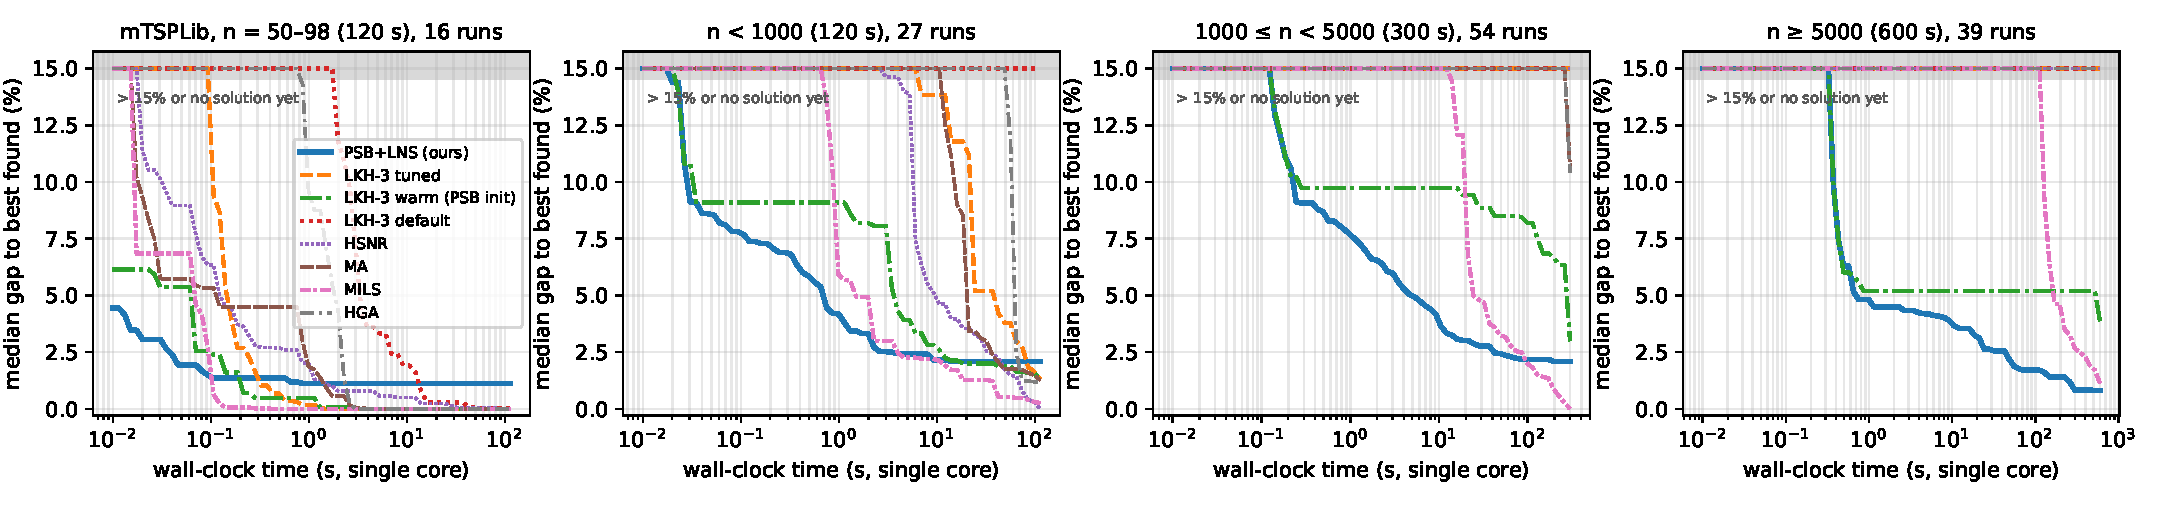
\includegraphics[width=\textwidth]{figs/fig_anytime.pdf}
\caption{Bulunan en iyi tamamlanma süresine göre medyan sapmanın duvar saati süresiyle
değişimi (tek çekirdek, logaritmik ölçek). Gölgeli bant: 15\% üzerinde sapma ya da henüz çözüm yok}\label{fig:anytime}
\end{figure}

\begin{table}[t]
\centering
\caption{Örnek boyutuna göre PSB+LNS ile literatürde öne çıkan kodların ve ayarlı LKH-3'ün
karşılaştırılması: ilk çözüme kadar geçen medyan süre ve bulunan en iyi tamamlanma süresine
göre medyan sapma (\%) ($\infty$: henüz çözüm yok). İlk çözüm medyanı yalnızca çözüm
döndüren koşuları, Wilcoxon testi iki yöntemin de sonlu nihai sonucu bulunan örnekleri
kapsar; büyük örneklerde HGA için test örneklem sayısı \SotaHgaWilcoxNLarge{}}\label{tab:sota}
\footnotesize
\setlength{\tabcolsep}{4pt}
\begin{tabular}{lrrrrrrr}
\toprule
method & first sol.\ [s] & 1\,s & 10\,s & 60\,s & final & PSB better [\%] & $p$ \\
\midrule
\multicolumn{8}{l}{\emph{$n<1000$, 43 instances}} \\
PSB+LNS (ours) & 0.01 & 2.43 & 1.77 & 1.63 & 1.63 & -- & -- \\
MILS & 0.08 & 3.58 & 1.12 & 0.01 & 0.00 & 23 & 3e-04 \\
HGA & 3.11 & \ensuremath{\infty} & 14.37 & 0.87 & 0.48 & 26 & 1e-02 \\
MA & 0.10 & 6.78 & 3.23 & 0.54 & 0.35 & 21 & 5e-03 \\
HSNR & 0.08 & 7.93 & 1.31 & 0.26 & 0.00 & 19 & 7e-03 \\
LKH-3 tuned & 2.04 & \ensuremath{\infty} & 2.10 & 0.86 & 0.57 & 28 & 6e-01 \\
\midrule
\multicolumn{8}{l}{\emph{$1000\le n<5000$, 54 instances}} \\
PSB+LNS (ours) & 0.10 & 7.70 & 3.82 & 2.29 & 2.08 & -- & -- \\
MILS & 4.73 & \ensuremath{\infty} & 23.04 & 2.90 & 0.00 & 17 & 4e-07 \\
HGA & 52.57 & \ensuremath{\infty} & \ensuremath{\infty} & \ensuremath{\infty} & 10.42 & 91 & 7e-10 \\
MA & 8.83 & \ensuremath{\infty} & 36.62 & 23.95 & 10.31 & 89 & 3e-09 \\
HSNR & 30.33 & \ensuremath{\infty} & \ensuremath{\infty} & 41.19 & 15.05 & 83 & 5e-09 \\
LKH-3 tuned & 244.97 & \ensuremath{\infty} & \ensuremath{\infty} & \ensuremath{\infty} & 31.53 & 85 & 2e-09 \\
\midrule
\multicolumn{8}{l}{\emph{$n\ge 5000$, 39 instances}} \\
PSB+LNS (ours) & 0.33 & 4.82 & 3.65 & 1.82 & 0.81 & -- & -- \\
MILS & 46.48 & \ensuremath{\infty} & \ensuremath{\infty} & 60.46 & 1.13 & 54 & 5e-01 \\
HGA & 1007.72 & \ensuremath{\infty} & \ensuremath{\infty} & \ensuremath{\infty} & \ensuremath{\infty} & 100 & 6e-02 \\
MA & 124.73 & \ensuremath{\infty} & \ensuremath{\infty} & \ensuremath{\infty} & 27.17 & 100 & 2e-10 \\
HSNR & 606.54 & \ensuremath{\infty} & \ensuremath{\infty} & \ensuremath{\infty} & 59.92 & 100 & 2e-06 \\
LKH-3 tuned & 600.87 & \ensuremath{\infty} & \ensuremath{\infty} & \ensuremath{\infty} & 97.14 & 100 & 4e-12 \\
\bottomrule
\end{tabular}

\end{table}

\paragraph{Küçük örnekler ($n<1000$)} Birkaç saniyeden fazla süre bulunduğunda bu
grupta klasik çözücüler tercih edilmelidir. MILS 60\,s sonunda 0.01\% medyan sapmaya
ulaşmış, PSB+LNS ise \CountSmall{} örneğin yalnızca \SotaMilsWinSmall\% kadarında MILS'ten
daha iyi sonuç vermiştir; ayarlı LKH-3 karşısındaki fark anlamlı bulunmamıştır
($p=\PvsTunedSmall$). PSB+LNS yalnızca ilk saniyelerde önde kalmıştır.

\paragraph{Orta büyüklükteki örnekler ($1000\le n<5000$)} PSB ilk çözümünü medyan 0.1\,s sonra,
MILS \SotaMilsFirstMid\,s sonra, MA, HSNR ve HGA 9 ile
53\,s arasında, ayarlı LKH-3 ise yaklaşık dört dakika sonra döndürmüştür. 10\,s anında
PSB+LNS, \CountMid{} örneğin \SotaMilsWinTenMid\% kadarında MILS'ten daha iyi sonuç vermiştir (MILS'in medyan sapması:
\SotaMilsTenMid\%). MILS yaklaşık iki dakika sonra PSB+LNS'yi geçmiş ve 300\,s'lik bütçenin
sonunda örneklerin çoğunda daha iyi sonuç vermiştir (PSB+LNS'nin daha iyi olduğu pay:
\SotaMilsWinMid\%). PSB+LNS, bütçe sonunda örneklerin 83--91\% kadarında HGA, MA, HSNR ve
ayarlı LKH-3'ten daha iyi sonuç vermiştir (tümünde $p<10^{-8}$).

\paragraph{Büyük örnekler ($n\ge 5000$)} 600\,s'lik bütçenin tamamı boyunca en düşük
medyan sapmayı PSB+LNS vermiştir. MILS ilk çözümünü medyan
\SotaMilsFirstLarge\,s sonra bildirmiş ve bütçe sonunda PSB+LNS ile başa baş kalmıştır
(\CountLarge{} örneğin \SotaMilsWinLarge\% kadarında PSB+LNS daha iyi, $p=\SotaMilsPLarge$); MA,
HSNR ve HGA çok geride kalmış, ayarlı LKH-3 ise hiçbir örnekte 60\,s içinde çözüm
bildirmemiş ve bütçeyi \TunedFinalLarge\% medyan sapmayla tamamlamıştır.

\InstAll{} örneğin tamamı üzerinde PSB+LNS, 1\,s sonunda örneklerin \SotaMilsWinOneAll\%
kadarında, 10\,s sonunda \SotaMilsWinTenAll\% kadarında ve bütçe sonunda \SotaMilsWinAll\%
kadarında MILS'ten daha iyi sonuç vermiştir; HGA, MA ve HSNR karşısındaki nihai paylar sırasıyla
\SotaHgaWinAll\%, \SotaMaWinAll\% ve \SotaHsnrWinAll\%, ayarlı LKH-3 karşısında ise
\WinFinalAll\% olmuştur ($p=\PvsTunedAll$). Nihai PSB+LNS sapma değerlerinin \SeedsMain{} tohum
arasındaki standart sapmasının medyanı \PsbSeedSdAll{} yüzde puan olmuştur.

\begin{table}[t]
\centering
\caption{PSB+LNS ve LKH-3: sabit bütçelerde, bulunan en iyi tamamlanma süresine göre medyan
sapma (\%) ($\infty$: henüz çözüm yok; çözüm bulunamayan koşuların payı
parantez içinde)}\label{tab:budget}
\footnotesize
\setlength{\tabcolsep}{4pt}
\begin{tabular}{lrrrrrr}
\toprule
method & 0.1\,s & 1\,s & 10\,s & 60\,s & cap & final \\
\midrule
\multicolumn{7}{l}{\emph{mTSPLib, 16 instances, cap 120\,s}} \\
PSB+LNS & 1.36 & 1.13 & 1.13 & 1.13 & -- & 1.13 \\
LKH-3 tuned & 9.39\,{\scriptsize(40\%)} & 0.17 & 0.00 & 0.00 & -- & \textbf{0.00} \\
LKH-3 warm & 2.54 & 0.47 & 0.00 & 0.00 & -- & 0.00 \\
LKH-3 default & \ensuremath{\infty}\,{\scriptsize(100\%)} & \ensuremath{\infty}\,{\scriptsize(69\%)} & 1.91 & 0.05 & -- & 0.01 \\
\midrule
\multicolumn{7}{l}{\emph{$n<1000$, 43 instances, cap 120\,s}} \\
PSB+LNS & 5.93 & 2.43 & 1.77 & 1.63 & -- & 1.63 \\
LKH-3 tuned & \ensuremath{\infty}\,{\scriptsize(78\%)} & \ensuremath{\infty}\,{\scriptsize(61\%)} & 2.10\,{\scriptsize(16\%)} & 0.86\,{\scriptsize(1\%)} & -- & 0.57 \\
LKH-3 warm & 8.16 & 6.51 & 1.78 & 0.44 & -- & \textbf{0.43} \\
LKH-3 default & \ensuremath{\infty}\,{\scriptsize(100\%)} & \ensuremath{\infty}\,{\scriptsize(88\%)} & \ensuremath{\infty}\,{\scriptsize(63\%)} & 30.48\,{\scriptsize(44\%)} & -- & 3.15 \\
\midrule
\multicolumn{7}{l}{\emph{$1000\le n<5000$, 54 instances, cap 300\,s}} \\
PSB+LNS & \ensuremath{\infty}\,{\scriptsize(48\%)} & 7.70 & 3.82 & 2.29 & 2.08 & \textbf{2.08} \\
LKH-3 tuned & \ensuremath{\infty}\,{\scriptsize(100\%)} & \ensuremath{\infty}\,{\scriptsize(100\%)} & \ensuremath{\infty}\,{\scriptsize(100\%)} & \ensuremath{\infty}\,{\scriptsize(84\%)} & 31.53 & 31.53 \\
LKH-3 warm & \ensuremath{\infty}\,{\scriptsize(52\%)} & 9.72 & 9.72 & 8.50 & 2.99 & 2.99 \\
LKH-3 default & \ensuremath{\infty}\,{\scriptsize(100\%)} & \ensuremath{\infty}\,{\scriptsize(100\%)} & \ensuremath{\infty}\,{\scriptsize(100\%)} & \ensuremath{\infty}\,{\scriptsize(100\%)} & 242.83\,{\scriptsize(30\%)} & 242.83 \\
\midrule
\multicolumn{7}{l}{\emph{$n\ge 5000$, 39 instances, cap 600\,s}} \\
PSB+LNS & \ensuremath{\infty}\,{\scriptsize(100\%)} & 4.82\,{\scriptsize(1\%)} & 3.65 & 1.82 & 0.81 & \textbf{0.81} \\
LKH-3 tuned & \ensuremath{\infty}\,{\scriptsize(100\%)} & \ensuremath{\infty}\,{\scriptsize(100\%)} & \ensuremath{\infty}\,{\scriptsize(100\%)} & \ensuremath{\infty}\,{\scriptsize(100\%)} & 97.14 & 97.14 \\
LKH-3 warm & \ensuremath{\infty}\,{\scriptsize(100\%)} & 5.20 & 5.20 & 5.20 & 3.87 & 3.87 \\
LKH-3 default & \ensuremath{\infty}\,{\scriptsize(100\%)} & \ensuremath{\infty}\,{\scriptsize(100\%)} & \ensuremath{\infty}\,{\scriptsize(100\%)} & \ensuremath{\infty}\,{\scriptsize(100\%)} & \ensuremath{\infty}\,{\scriptsize(85\%)} & \ensuremath{\infty} \\
\bottomrule
\end{tabular}

\end{table}

LKH-3'ün PSB çözümünden sıcak başlangıçla çalıştırılması, ilk tur için gereken uzun bekleme süresini ortadan
kaldırmıştır; ancak Şekil~\ref{fig:anytime} üzerindeki eğrilerinde görülen düz kesimler, bütçenin
büyük kısmının başlangıç çözümü iyileştirilmeden geçtiğini göstermektedir. Bütçe
sonunda PSB+LNS, orta büyüklükteki örneklerin \WinWarmMid\% kadarında ve büyük örneklerin
\WinWarmLarge\% kadarında sıcak başlangıçlı LKH-3'ten daha iyi sonuç vermiştir.

\subsection{Kurulum süresi, ölçeklenme ve paralellik}
LNS olmadan PSB, medyan \PsbOneShotMs\,ms sonra, bulunan en iyi tamamlanma süresine göre
medyan sapması \PsbOneShotGap\% olan bir çözüm döndürmüştür; ayarlı LKH-3 ise örneklerin
\ReachNeverAll\% kadarında bütçesi içinde bu kaliteye ulaşamamıştır. Tek atış
süresi $n$ ile neredeyse doğrusal olarak artmıştır (uydurulan üs \ScaleExponent;
$n=\ScaleNLargest$ için \ScaleMsLargest\,ms). Rota başına hesaplama çekirdeklerinin dört
veya daha fazla iş parçacığında çalıştırılması kurulumu hızlandırmamış, aksine yavaşlatmıştır
(medyan hızlanma \ScaleSpeedupFour); bunun nedeni, dev tur ve bölme adımlarının hesaplama süresine
hâkim olması ve sıralı yürütülmesidir. Bu nedenle tüm sonuçlarda tek çekirdek kullanılmıştır.

\subsection{Ablasyon}
Tablo~\ref{tab:ablation}, her seferinde bir bileşen çıkarılarak ya da değiştirilerek elde
edilen medyan tek atış tamamlanma süresini tam işlem hattına göre vermektedir. Dengeleme
yaklaşık 2\% (tüm örnekler üzerinde \AblNoBalanceAll\%), optimal bölme eşit uzunluklu
bölmeye karşı \AblEqualSplitAll\%, dev tur üzerindeki yerel arama ise yaklaşık 1.5\%
katkı sağlamıştır. Önce küme, sonra rota yaklaşımına dayalı alternatifler belirgin biçimde daha kötü sonuç vermiştir:
her küme için ayrı bir TSP çözülen $k$-means yaklaşımı \AblKmeansTspAll\%, PSB dengeleme adımı eklendiğinde
bile \AblKmeansBalAll\% kayba yol açmıştır. Depo çevresinde açısal tarama, düzenli
sentetik bahçelerde PSB'ye çok yakın bir medyan vermiş (\AblSweepTspOrchard\%), ancak gerçek
bahçe sınırlarında \AblSweepTspOsm\%, VLSI örneklerinde ise \AblSweepTspVlsi\% kayba yol açmıştır;
30\,s'lik LNS sonrasında başlangıç seçiminin etkisi küçük kalmıştır (tarama
başlangıcı için \LnsStartOrchard\% ve \LnsStartVlsi\%). Bu bulgu, kurulum adımının asıl katkısının
erken aşamada iyi bir çözüm sağlamak olduğunu göstermektedir.

\begin{table}[t]
\centering
\caption{Tek atış kurulum adımının ablasyonu: tam PSB işlem hattına göre medyan tamamlanma süresi
(\%) ve medyan süre; sent.: sentetik bahçeler, gerçek: gerçek
bahçe sınırları, lit.: literatür kümesi (örnek sayıları parantez içinde)}\label{tab:ablation}
\scriptsize
\setlength{\tabcolsep}{2.5pt}
\begin{tabular}{lrrrrrr}
\toprule
variant & mTSPLib (16) & synth. (48) & real (48) & VLSI (24) & lit. (52) & time [ms] \\
\midrule
PSB (full) & -- & -- & -- & -- & -- & 80 \\
no Balance & +2.70 & +1.82 & +2.31 & +1.68 & +2.58 & 44 \\
no Polish, no Balance & +4.25 & +2.28 & +2.43 & +1.84 & +2.76 & 26 \\
equal-length split & +0.00 & +1.06 & +1.34 & +5.54 & +4.12 & 106 \\
GE tour, no 2-opt/Or-opt & +1.20 & +1.35 & -0.17 & +1.67 & +1.62 & 87 \\
nearest-neighbour tour & +0.25 & +0.75 & +0.63 & +1.11 & +0.13 & 186 \\
sweep + TSP & +1.55 & +0.09 & +6.37 & +6.30 & +3.68 & 33 \\
$k$-means + TSP & +13.03 & +26.03 & +26.44 & +20.49 & +20.56 & 35 \\
$k$-means + TSP + Balance & +2.70 & +11.67 & +13.61 & +7.48 & +5.78 & 101 \\
\bottomrule
\end{tabular}

\end{table}

\subsection{Literatür kıyaslaması}
Ek~A, $\mathbb{S}$ ve $\mathbb{L}$ kümelerindeki
\LitCount{} örneğin referans değerlerine göre sapmalarını listelemektedir. Referans değerler
birkaç saate kadar süren koşulardan elde edilmiştir \citep{hehaoxia2024}; burada ise en
fazla 600\,s süren tek bir koşu yapılmıştır. PSB+LNS hiçbir referans değeri iyileştirmemiştir.
Az sayıda robotun kullanıldığı örneklerde ($k\le 5$, \LitFewKCount{} örnek) PSB+LNS'nin medyan sapması
\LitFewKPsbFinal\% olmuş, bu değer MILS için \LitFewKMilsFinal\%, ayarlı LKH-3 için
\LitFewKTunedFinal\% olarak bulunmuştur; çok sayıda robotun kullanıldığı örneklerde ($k\ge 10$) ise medyanlar sırasıyla
\LitManyKPsbFinal\%, \LitManyKMilsFinal\% ve \LitManyKTunedFinal\% olmuştur. Her iki grupta
da bütçe sonunda en düşük sapmayı MILS sağlamış, PSB+LNS ise çok sayıda robot içeren
\LitManyKCount{} örneğin \LitManyKPsbBeatsTuned{} tanesinde ayarlı LKH-3'ten daha iyi
sonuç vermiştir.

\subsection{Mutlak kalite}
Nihai PSB+LNS tamamlanma süresinin alt sınır~\eqref{eq:lb} değerine göre medyan sapması
sentetik bahçelerde \LbGapOrch\%, VLSI örneklerinde \LbGapVlsi\% ve mTSPLib örneklerinde
\LbGapMtsp\% olmuştur; bu farkın bir kısmı, ne en uzak hedef teriminin ne de MST teriminin baskın
olduğu durumlarda sınırın zayıf kalmasından kaynaklanmaktadır.
